\section{How can we Slow down Aging?}

\subsection{Overview}

\begin{frame}[c]{Goal of Anti-Aging Research}
    \large
    As I understand it, the goal of anti-aging research is \textbf{the extension of the human lifespan}.

    Ideally by stopping aging or achieving neglegible senescence.
    Intermediate goals include slowing down aging, and increasing QUALYs
    (QUality-Adjusted-Life-Years).
    \pnote{
        neglegible senescence = not aging biologically \\
        \par
        neglegible senescence is further out, we are \\
        barely able to slow it down a few percent \\
        \par
        aim for longevity escape velocity
    }
\end{frame}

\begin{frame}[c]{Potential Strategies to Slow down Aging}
    \scriptsize
    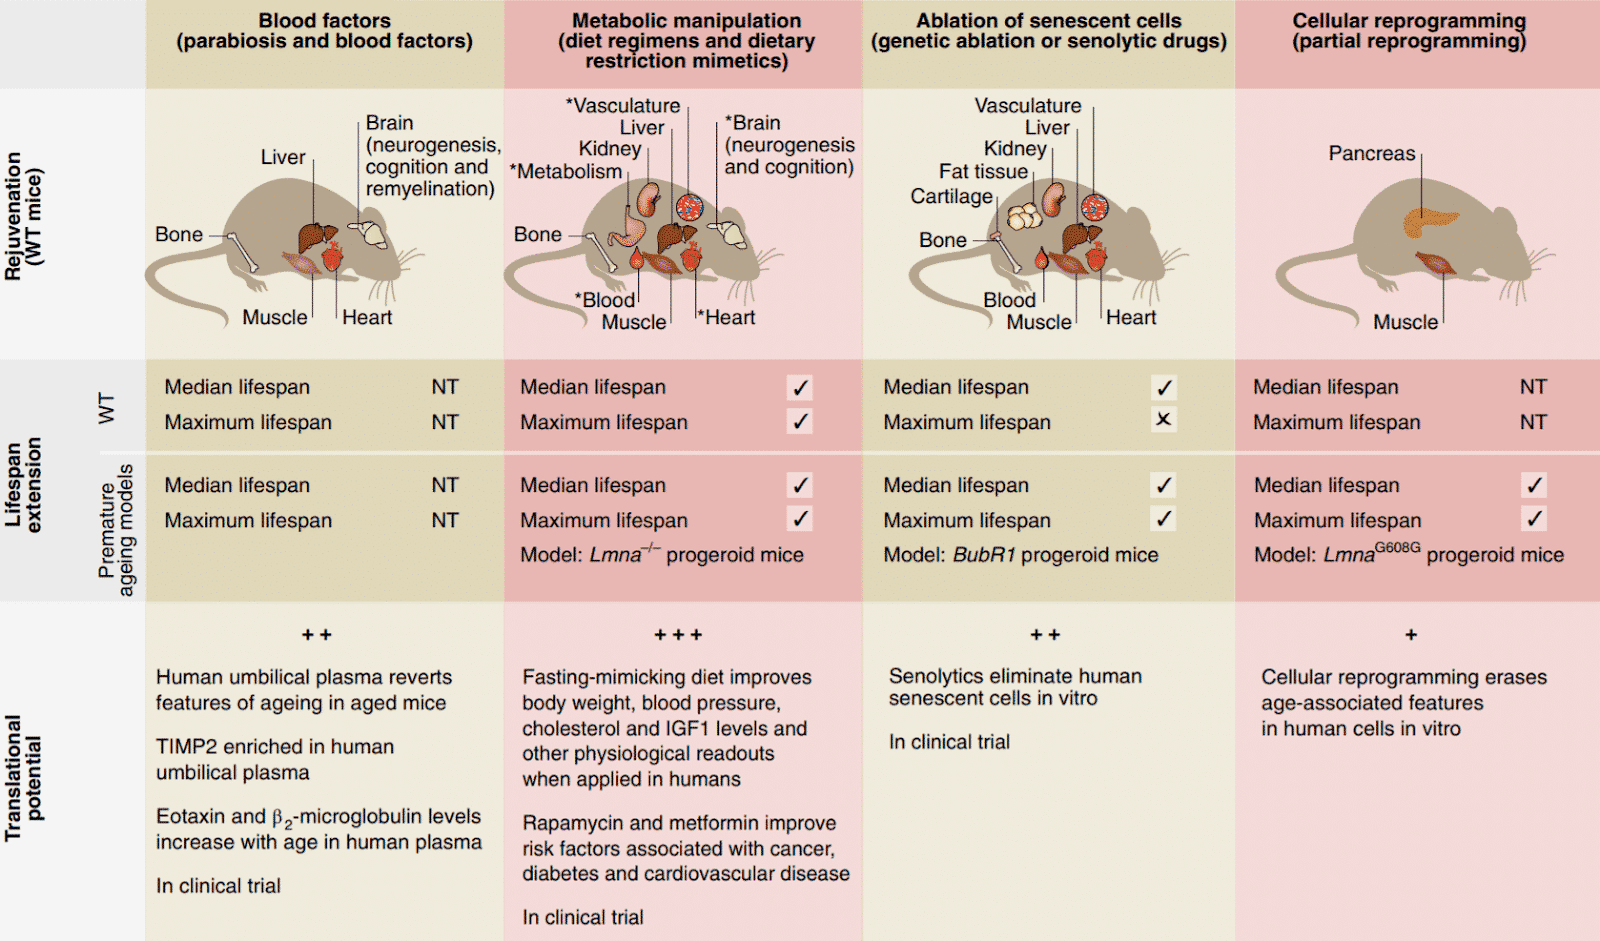
\includegraphics[width=\textwidth,clip,trim=0 280 0 0]{strategy_comparison_short} \\
    Source: \cite{mahmoudi2019turning}, picture modified

    \pnote{
        Comparison of rejuvenation strategies \\
        Currently highest potential, but more exist
        \par
        We will take a deeper look at all of them \\
        No need to study overview for long
        \par
        Treatment initiated midlife or later \\
        \par
        Next: Parabiosis
    }
    % go real in-depth on two topics, don't spread too much
    % remove parabiosis and either cellular reprogramming (since epigenetics first) or senolytics

    % \pnote{A comparison of the four emerging rejuvenation strategies: blood factors,
    % metabolic manipulation, ablation of senescent cells and cellular
    % reprogramming. The figure depicts the features that improve when treatment
    % in mice is initiated at midlife or later. The top panel shows organs or
    % tissues that exhibit a rejuvenated phenotype in wild-type (WT) mice. For
    % rapamycin, features that have been shown to improve also in young mice
    % following treatment are indicated with an asterisk (*). The effect on
    % lifespan, proposed primary mode (or modes) of action and possible
    % trade-offs of these strategies are also presented. Finally, the
    % translational potential in humans is indicated by the increasing number of
    % plus signs (+) based on present evidence in human ageing and current
    % feasibility. NT, not tested. Question marks indicate possible modes of
    % action and trade-offs.}
\end{frame}



\subsection{Metabolic Manipulation}

\begin{frame}[c]{Dietary Restriction in D. melanogaster (Fruit Fly)}
    \scriptsize
    % trim = l b r t
    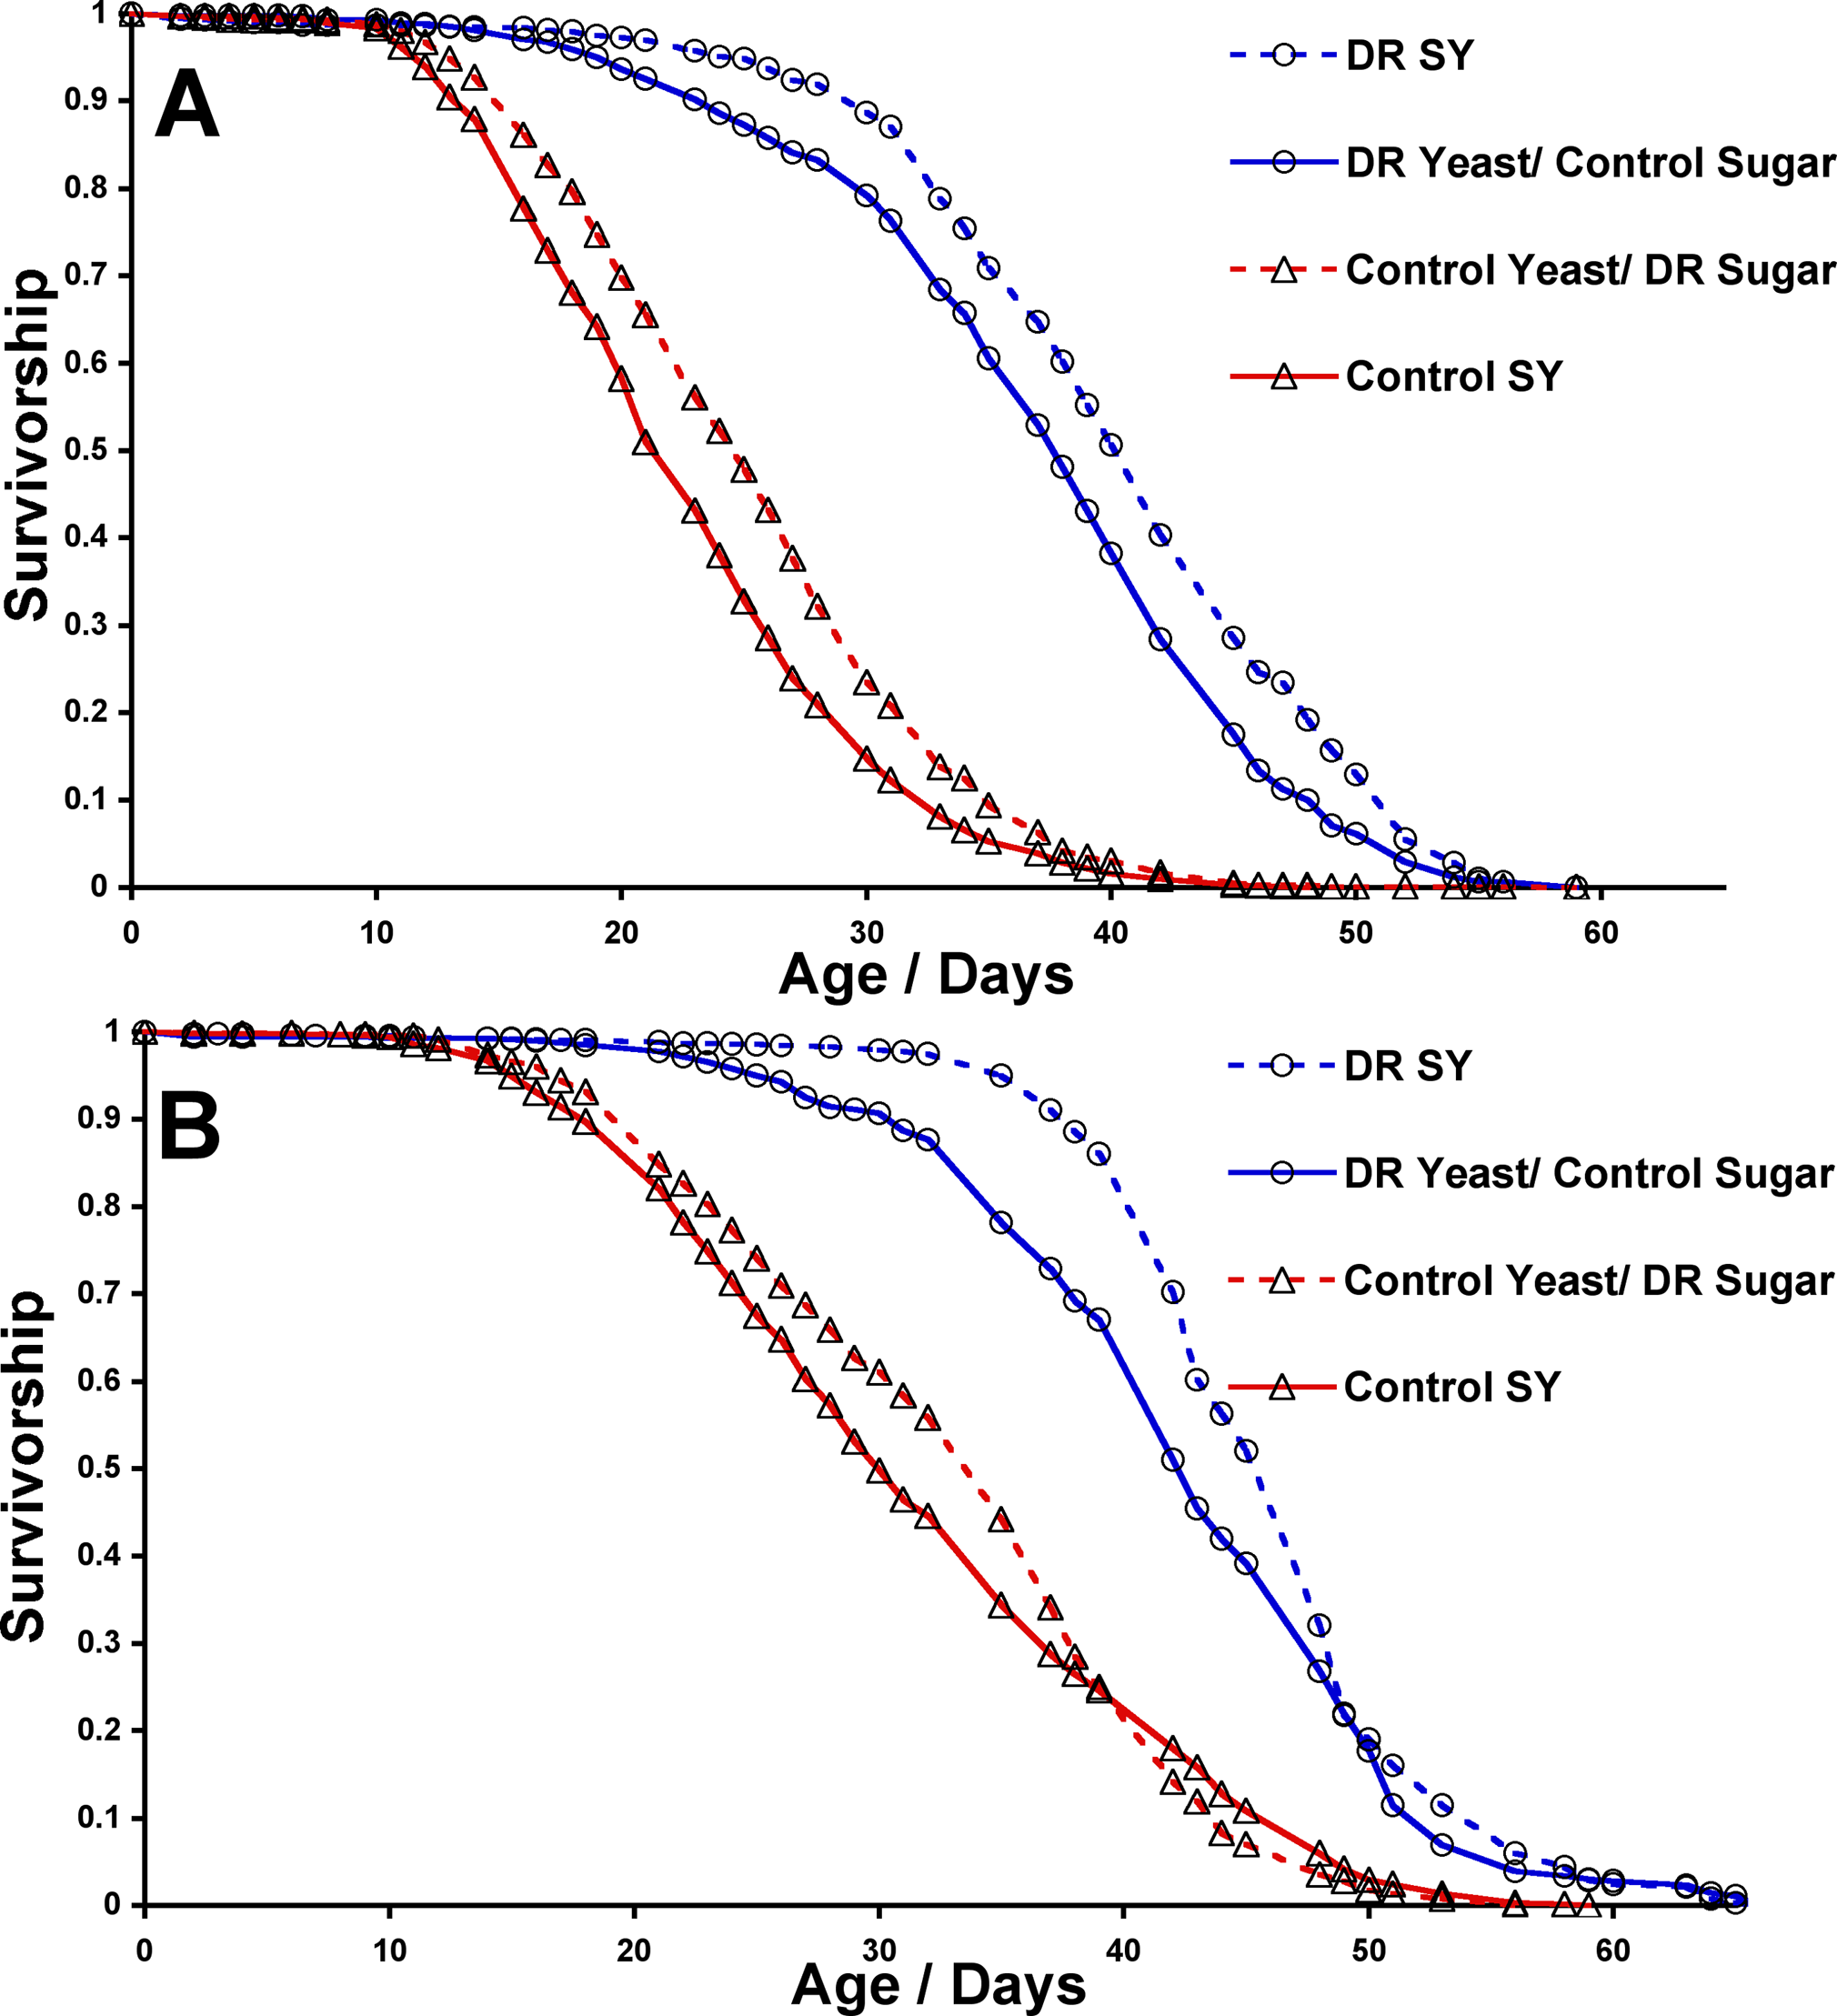
\includegraphics[width=\textwidth,clip,trim=0 57 0 0]{cr_lifespan_increase} \\
    Source: \cite{mair2005calories}
    \small
    \begin{multicols}{2}
    \begin{itemize}
        \item DR = Dietary Restriction
        \item Control = No Restriction
        \item S = Sugar
        \item Y = Yeast
    \end{itemize}
    \end{multicols}
    \pnote{
        Originally caloric restriction \\
        Experiment showed: not just calories \\
        Has been replicated as well \\
        Lifespan increase 20-40\% \\
        A/B replication of same setup
        \par
        Visible: does not just depend on calories \\
        Also well-established in Humans
        \par
        Next: Why does this work? What does it do? \\
    }
\end{frame}


\begin{frame}[c]{Dietary Restriction Effects}
    \large
    \begin{itemize}[<+(1)->]
        \item 'Different' mitochondrial energy production (less Reactive Oxygen Species, ROS)
        \item Reduced protein synthesis and DNA duplication
        \item Increased repair capacity (SIRT and others)
        \item Increased removal of misfolded proteins (Autophagy)
        \item Reduced inflammation and proliferation
    \end{itemize}
    \pause
    Overall: Optimizing energy and resource usage
    \pnote{
        ROS = Reactive Oxygen Species, damage-inducing \\
        Usual mode: just blast through / press ahead \\
        "Ohne Rücksicht auf Verluste" \\
        Less safety checks and enthusiastic production
        \par
        Works, as usually enough energy is present \\
        Also: Mitochondrial downregulation \\
        Proliferation: cell division and protein synthesis
        \par
        Maybe we can target these pathways directly? \\
        Next: Inhibiting mTOR receptors
    }
\end{frame}



\begin{frame}[c]{Metformin Effects}
    \scriptsize
    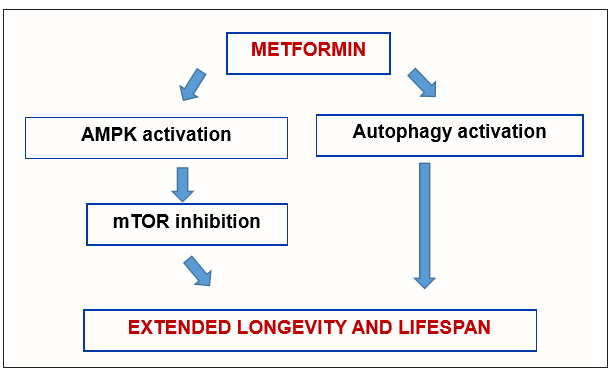
\includegraphics[width=\textwidth]{metformin_effects} \\
    Source: \cite{podhorecka2017metformin}
\end{frame}

\begin{frame}[c]{Method Evaluation: Metabolic Manipulation}
    \textbf{Hallmarks affected}: \\
    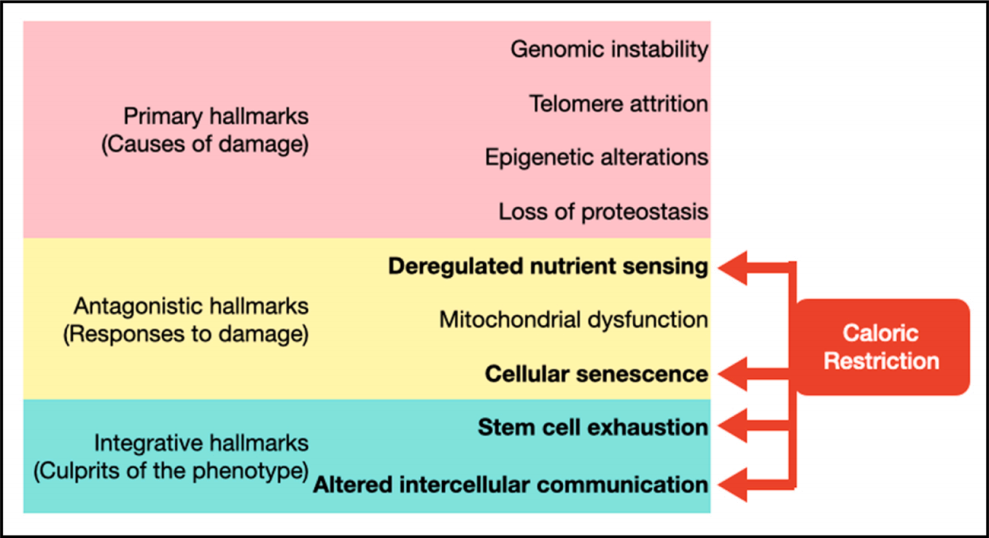
\includegraphics[width=0.7\textwidth]{cr_pathway_effects}
    % \begin{itemize}[<+(1)->]
    %     \item Deregulated Nutrient Sensing
    %     \item Cellular Senescence
    %     \item Stem Cell Exhaustion
    %     \item Altered Intercellular Communication
    % \end{itemize}
    \scriptsize
    Source: \cite{erbaba2020effects} \\
    \normalsize
    \pause
    Lifespan extension: about 20-40\% QUALY \cite{swindell2012dietary} \\
    \pause
    \textbf{State: In clinical trial}, e.g. \cite{TAMETarg47:online}
    \pnote{
        More of a 'slow down', preventing worst case \\
        Not silver bullet, rather 'one-trick pony' \\
        Not clear that this is correct classification
        \par
        Not 'root-cause' prevention \\
        but still amazing progress \\
        \par
        Next: Senolytics
    }
\end{frame}


\subsection{Senolytics}

\begin{frame}[c]{Senescent Cells: What are they?}
    \large
    \begin{itemize}[<+(1)->]
        \item `Zombie-like death-resistent cells'
        \item Old or (partially) damaged cells
        \item Sending out Senescence-Associated Secretory Phenotype (SASP)
        \item SASP disrupts intercellular communication, causing inflammation and age-related diseases
        \item Cells manage to induce apoptosis (cell-suicide) or get removed by the immune system
        \item About 8\% of cells in young, and 17\% of cells in old mice are senescent \cite{folgueras2018mouse}
    \end{itemize}
    \pnote{
        SASP part of damage-fallback state \\
        'I won't be able to fix this' \\
        Severely disrupts intercellular communication
        \par
        Very interesting: senescent difference \\
        in old vs young mice \\
        \par
        Next: Senolytics Effects
    }
\end{frame}


% \begin{frame}[c]{Senescent Cell Effects}
%     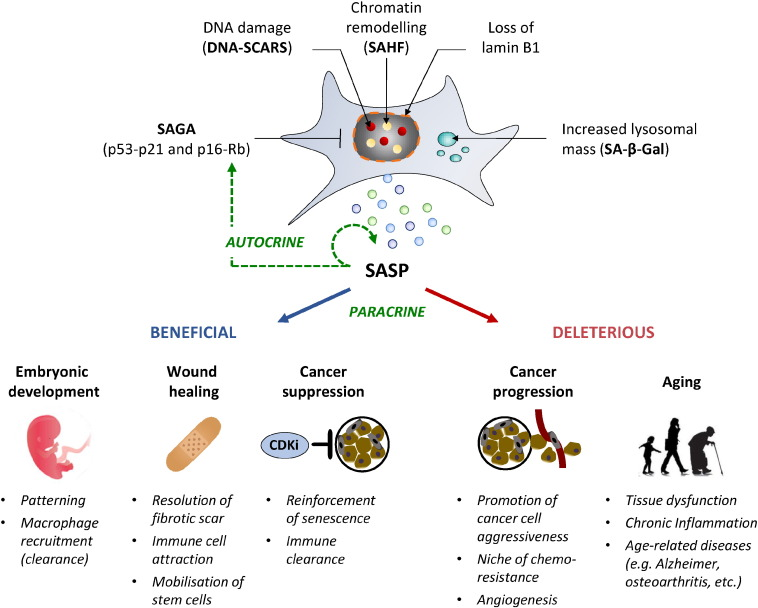
\includegraphics[height=0.85\textheight]{sasp_effects} \\
%     Source: \cite{malaquin2016keeping}
%     \pnote{
%         SASP meant to increase cell-turnover \\
%         more apoptosis, more cell growth to replace \\
%         less 'safety checks' with high proliferation
%         \par
%         also toxic agents + ROS to make less hospitable \\
%         specific factors induce cell death and growth
%         \par
%         good for wound healing (high turnover) \\
%         Klassisch: 'Entzündung' (inflammation)
%         \par
%         Next: Senolytic Uses and Effects
%     }
% \end{frame}


% \begin{frame}<handout>[c]{Inflammation Effects}
%     \begin{aquote}{\cite{NintilTh68:online}}
%         {\em Also, the environment that inflammation creates is one that is} meant to
%         increase cell turnover {\em (More apoptosis, but also more cell growth to
%         replace lost cells), with granulocytes secreting toxic agents
%         (Including ROS) to make the area affected less hospitable (But also
%         increases damage to DNA), and specific cytokines like the} tumor
%         necrosis factor that induce cell death, and growth factors that promote
%         cell growth.
%     \end{aquote}
% \end{frame}


\begin{frame}[c]{Senolytics and Aged Cells}
    \scriptsize
    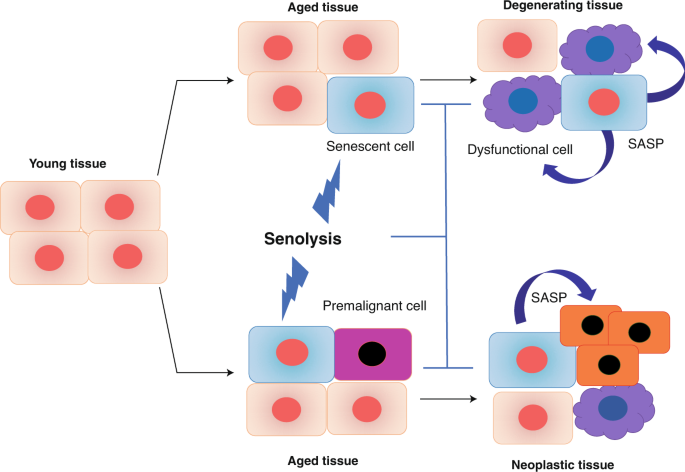
\includegraphics[height=0.85\textheight]{senolytics_effect}
    Source: \cite{dolgin2020send}
    \pnote{
        SASP has negative effects on neighbouring cells \\
        disrupting intercellular communication \\
        ground for cell-turnover -> tumorgenesis \\
        awesome machanism for healthy tissue!
        \par
        Senolytics 'help Senescent cells to die' \\
        (euthanasia) or modulate SASP damage
        \par
        Next: Senolytics Evaluation
    }
\end{frame}

% \begin{frame}[c]{Senolytics (Drugs killing senescent cells)}
%     Senescent cells are a kind of 'zombie'-like cell that accumulate with age. They are death-resistant cells that secrete proinflammatory factors associated with a range of age-related diseases (below, right):

% Cellular senescence is associated with multiple human disorders. The development of galactose‐conjugated and fluorescent probes to detect and highlight senescent cells offers an important opportunity for longitudinal monitoring of senescence in clinical trials. Pharmacologically active small compounds known as senolytics inhibit pro‐survival pathways in senescent cells leading to apoptosis, a therapeutic strategy that may additionally be enhanced by the use of immune modulators promoting natural clearance of senescent cells. Finally, nanoparticles encapsulating cytotoxic drugs, tracers and/or small molecules can be used as theranostic tools, both for therapeutic and diagnostic purposes. Source: here
% There are various strategies being explored to kill or reprogram senescent cells (above, left), including senolytics. Senolytics are drugs that kill senescent cells to improve physical function and healthy lifespan. When administered to older mice, senolytics have been shown to reverse many aspects of aging such as cataracts, and arthritis (below):

% Killing senescent cells with senolytics extends the median healthy lifespan by up to 27\% in mice (below). Several senolytics, such as the combination of dasatinib and quercetin, and fisetin are in clinical trials in humans today.

% Study design for clearance of senescent cells mouse cohort. Median survival (in days, d) and percentage increase in median survival are indicated. Source: here
% Hallmarks of aging reversed: senolytics decelerate cellular senescence, improve epigenetic markers and restore intercellular communication (by reducing inflammation associated with senescent cells) to extend healthy lifespan.
% \end{frame}


\begin{frame}[c]{Method Evaluation: Senolytics}
    \textbf{Hallmarks affected}: \\
    \begin{itemize}[<+(1)->]
        \item Decelerate Cellular Senescence
        \item Improve Epigenetic Markers
        \item Restore Intercellular Communication (by reducing inflammation associated with senescent cells)
    \end{itemize}
    \pause
    Lifespan extension: 27\% median Life\\
    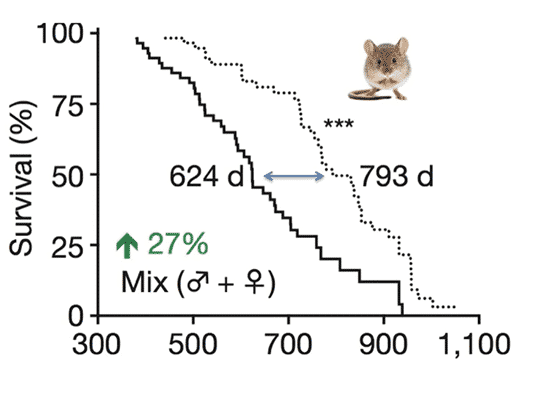
\includegraphics[width=0.4\textwidth]{senolytics_extend_life}
    \scriptsize
    Source: \cite{baker2016naturally} \\
    \normalsize
    \pause
    \textbf{State: In clinical trial}
    \pnote{
        Going much more in on root causes \\
        Depends heavily on immune system capacity \\
        \par
        Bonus: Very different mechanism, \\
        so probably good complement to other methods \\
        \par
        Next: Cellular Reprogramming
    }
\end{frame}


\subsection{Other Approaches}

\begin{frame}[c]{Other Promising Approaches}
    \large
    \begin{itemize}[<+(1)->]
        \item Blood Exchange (Parabiosis) \cite{conese2017fountain}
        \item Cellular Reprogramming \cite{ocampo2016vivo}
        \item Thymic (Immune System) rejuvenation \cite{fahy2019reversal}
        \item Sirtuin activation for DNA repair \cite{mohar2012sirtuin}
        % \item Boosting mitochondrial function with NAD+ precursor molecules \cite{aman2018therapeutic}
        % \item Identifying genetic Markers \cite{kenyon2010genetics}
        \item Many more ...
    \end{itemize}
    \pnote{
        SIRT are part of DNA damage repair pathways \\
        NAD is being consumed in emergency response \\
        NAD = Nicotinamide adenine dinucleotide \\
        Preventing dangerous mitochondrial fail-states \\
        Unclear how genetic markers affect longevity
        \par
        Next: Evaluation
    }
\end{frame}


% \begin{frame}[c]{Method Evaluation: Other Approaches}
%     \large
%     \textbf{Hallmarks affected}: ??? \\
%     \pause
%     Lifespan extension: Most 5\%-40\% \\
%     \pause
%     State: Active research, some in animal or clinical trials
%     \pnote{
%         A lot of different approaches \\
%         Many with as-yet-unknown effects on vertebrates \\
%         yet others already in clinical trials \\
%         All of what I'm presenting is active research
%         \par
%         Ask me about state of yeast
%         \par
%         Next: What can I do?
%     }
% \end{frame}
